\chapter{Extra Results}

\section{WMT NewsTest profiling using one GPU}
\label{appendix:result:bytenet-profile}

\begin{figure}[h]
    \centering
    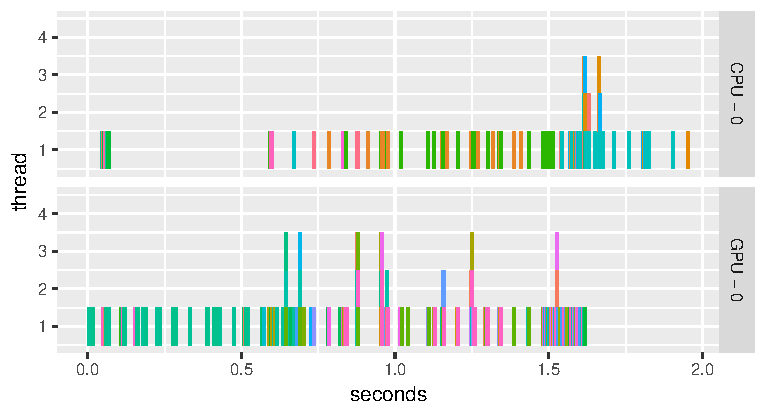
\includegraphics[width=\textwidth]{bytenet/profile-raw-gpu1.pdf}
    \caption{Shows time spend on each operation, when the operation was executed, and on what GPU/CPU it was executed. The color coding indicates the operation type, there are more than a 100 diffrent operation types, most are specific to TensorFlow, thus the legend is not included.}
\end{figure}

\begin{figure}[h]
    \centering
    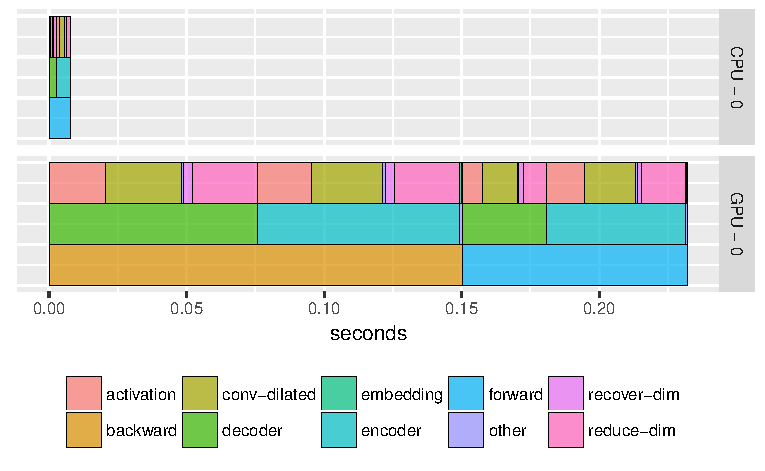
\includegraphics[scale=1]{bytenet/profile-grouped-gpu1.pdf}
    \caption{Shows time spend executing operations in each part of the ByteNet model, this excludes the waiting time. Each part exists in a hierarchy, which is visualized as levels. The bottom level is the least detailed level, it just splits the model in the backward and forward pass. The next level, splits the model in the encoder and decoder. The last level at the top, primarily splits the ByteNet Residual Blocks.}
\end{figure}
